\begin{figure}
% 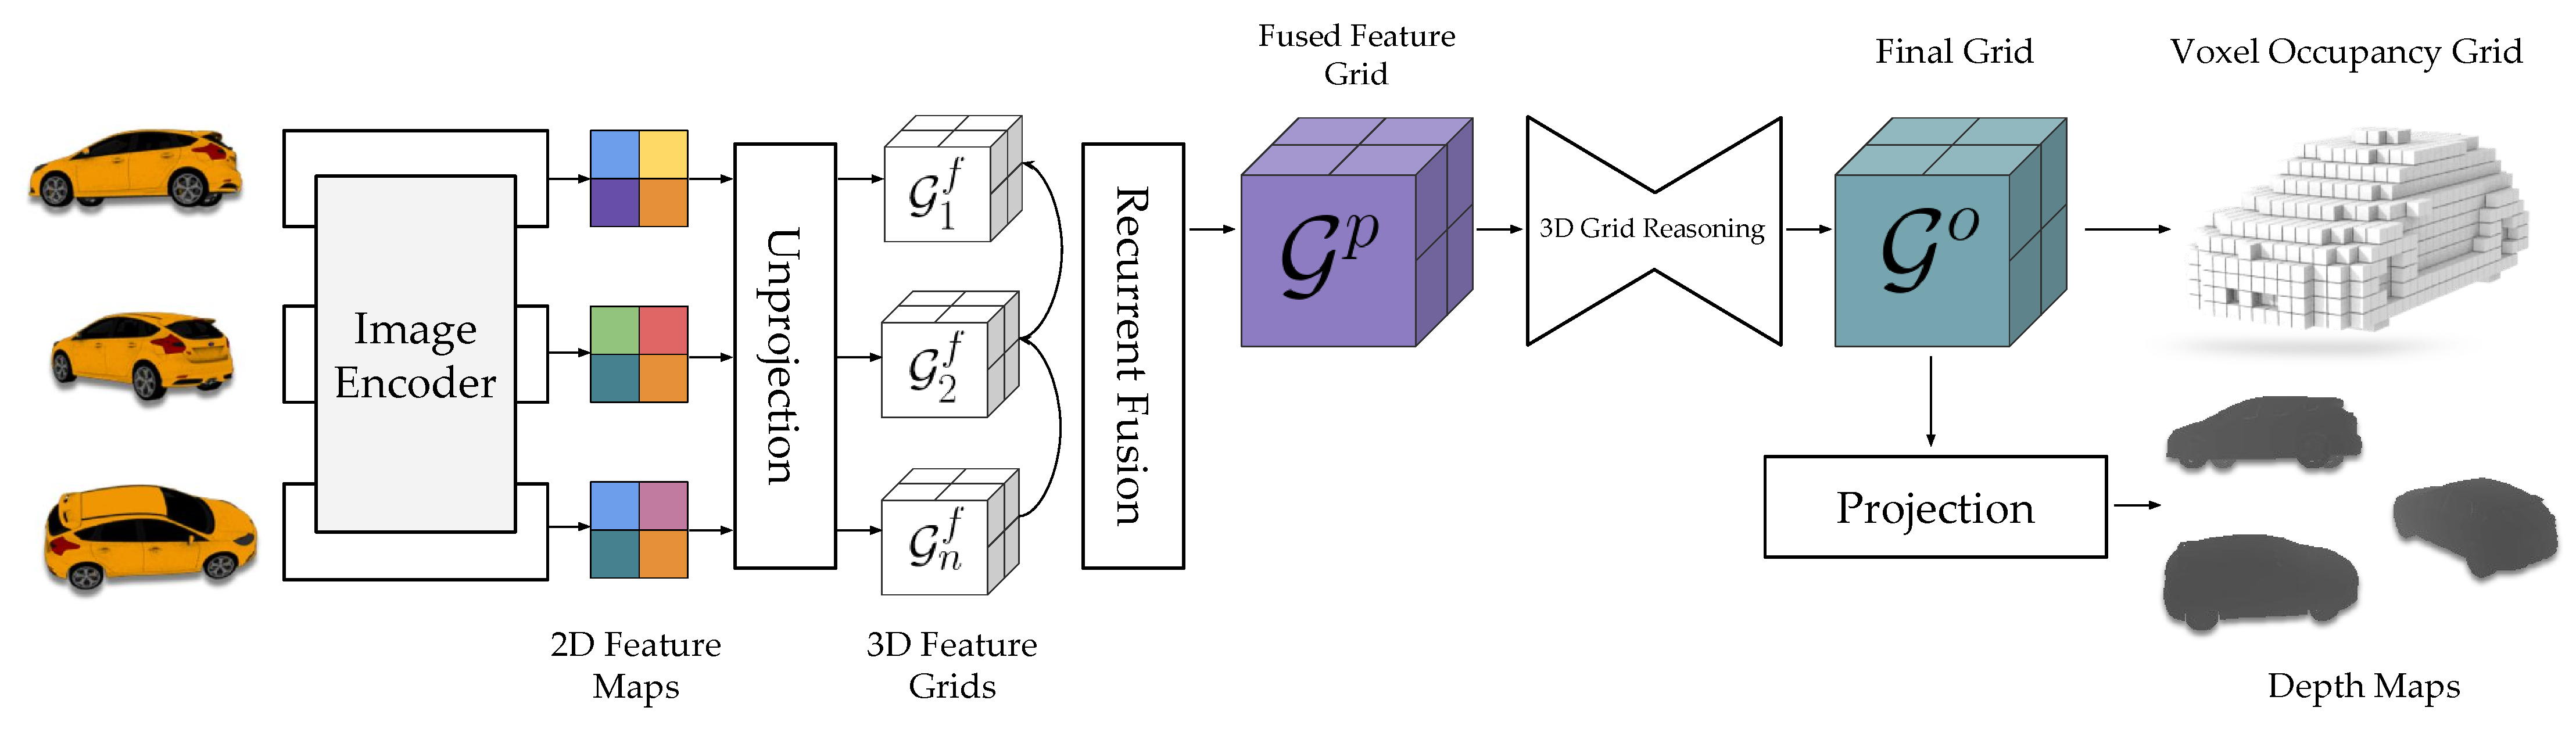
\includegraphics[width=\linewidth]{figures/lsm/overview.pdf}
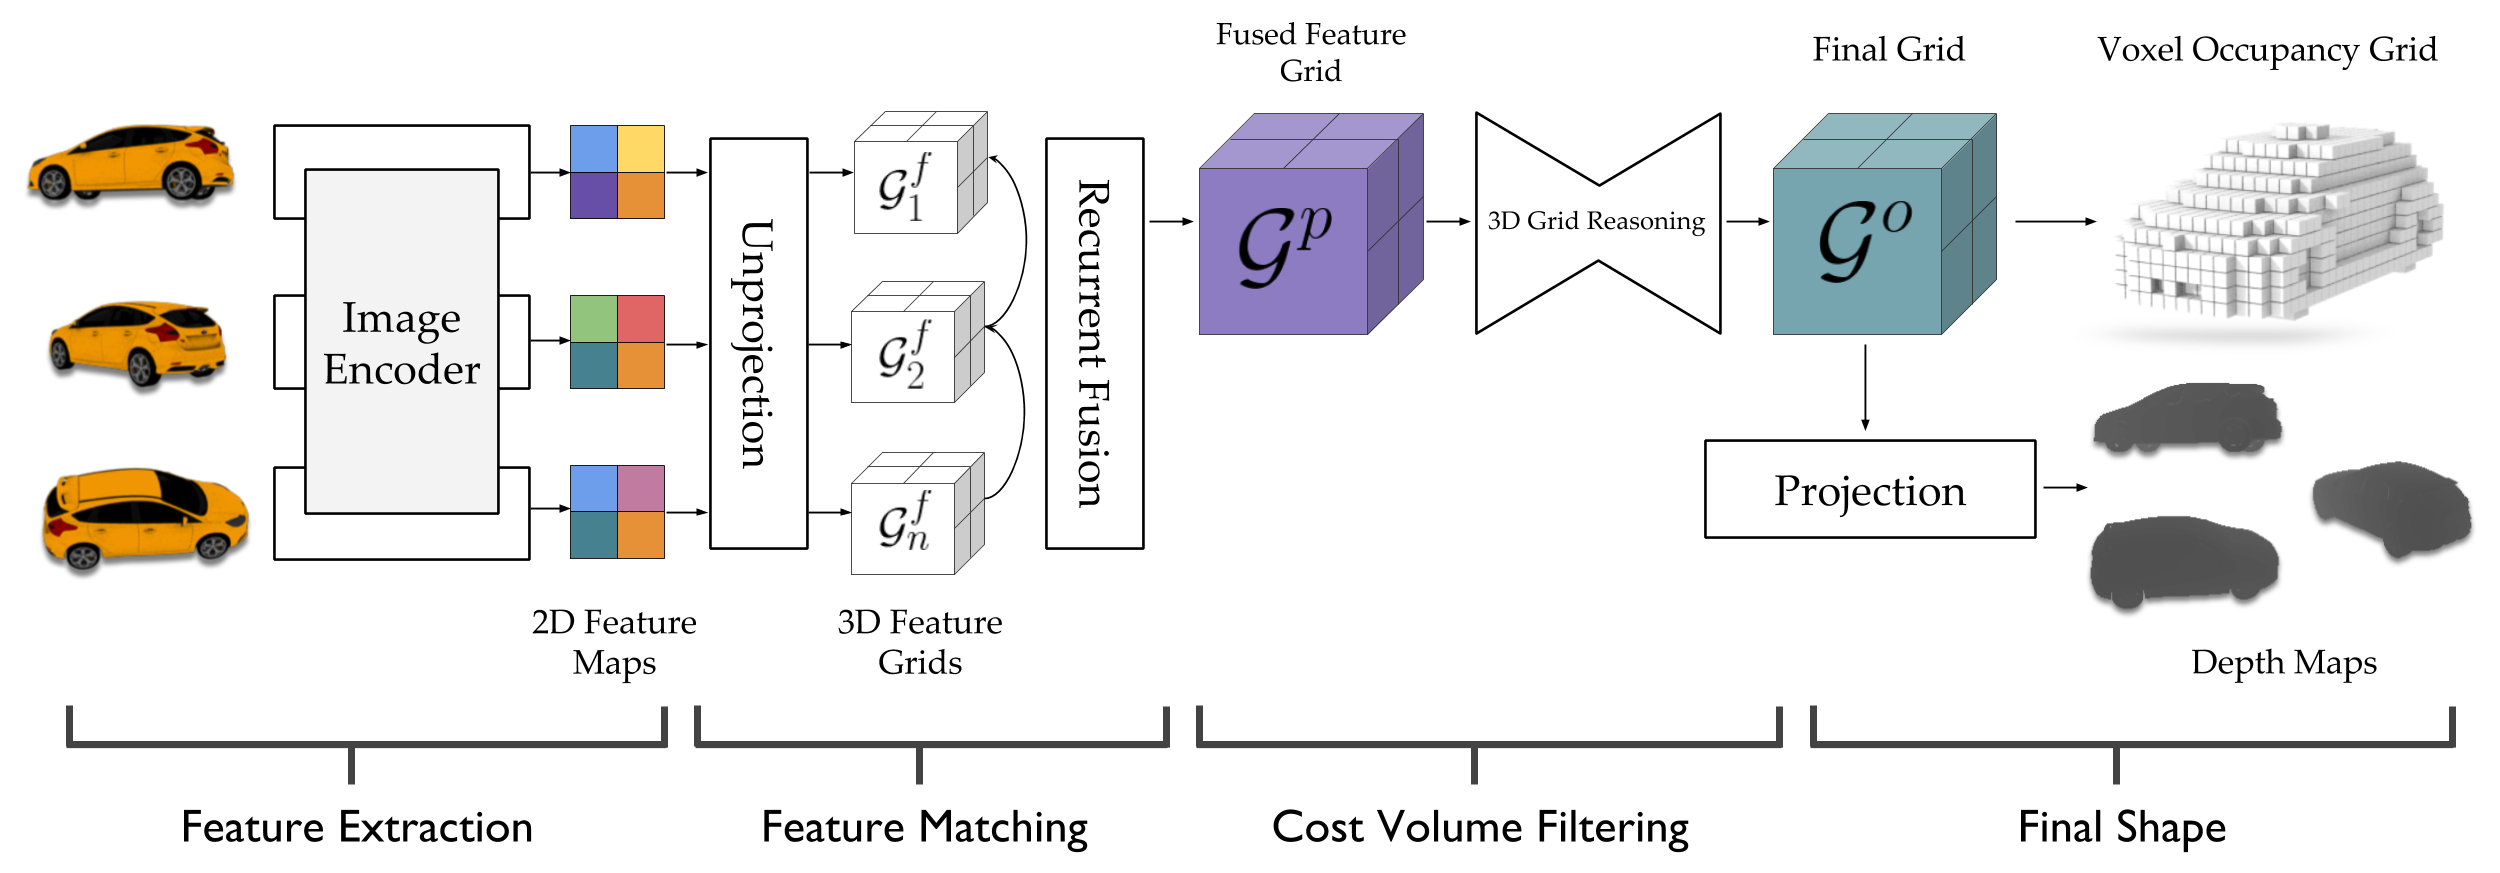
\includegraphics[width=\linewidth]{figures/lsm/overview2.png}
\caption{Overview of a Learnt Stereo Machine (LSM). It takes as input one or more views and camera poses. The images are processed through a feature encoder which are then unprojected into the 3D world frame using a differentiable unprojection operation. These grids $\mc\{{G}^f_i\}_{i=1}^n$ are then matched in a recurrent manner to produce a fused grid $\mc{G}^p$ which is then transformed by a 3D CNN into $\mc{G}^o$. LSMs can produce two kinds of outputs - voxel occupancy grids (Voxel LSM) decoded from $\mc{G}^o$ or per-view depth maps (Depth LSM) decoded after a projection operation.} 
\figlabel{overview}
\end{figure}